\documentclass[12pt]{beamer}
\usetheme{CambridgeUS}
\usecolortheme{lily}
\usepackage{extsizes}
\usepackage{amsmath}
\usepackage{setspace}
\usepackage{commath}
\usepackage{graphicx}
\geometry{margin=0.125in}
\title{debuginfod}
\subtitle{and its interaction with the 
Yocto Project}
\author{Dylan Garza}
\date{\today}

\begin{document}

\frame{\titlepage}

\begin{frame}
   \frametitle{ debuginfod}
   \begin{itemize}
      \item What is debuginfod?
      debuginfod is a daemon turns a machine that
      holds debug artifacts into file server for
      easier debugging. Tools such as gdb, valgrind, and systemtap utilize 
         debuginfod. \\
      \vspace{.5cm}
      \item Why use it?
      Debug info is too big to be stored locally
      on the target devices. Different versions 
      of binaries exist, so corresponding debug info is fethced automatically 
      with gdb. 
   \end{itemize}
\end{frame}

\begin{frame}[fragile]
   \frametitle{ Installing debuginfod}
   \vspace{-1cm}
   \noindent
   There are two ways to install on a Ubuntu machine:
   \begin{itemize}
      \item Upgrade to Ubuntu 22.04
      \item append the "impish" package to \color{gray}\verb|/etc/apt/sources.list|
         \color{black} by appending the following line:
   \end{itemize}
   \color{gray}
   \fontsize{8pt}{10pt}{\selectfont}
   \begin{verbatim}
   deb http://archive.ubuntu.com/ubuntu impish main restricted universe multiverse
   \end{verbatim}
\end{frame}

\begin{frame}[fragile]
   \fontsize{8pt}{10pt}{\selectfont}
   \frametitle{ Setting up and using debuginfod}
   Starting the debuginfod server:
   \begin{itemize}
      \item To start the file server, simply run \verb|debuginfod -F|. 
         Different arguments will search for different debug artifacts (\verb|-F -R -U|)
         \begin{itemize}
         \fontsize{8pt}{10pt}{\selectfont}
            \item -F sets file scanning for ELF/DWARF artifacts.
            \item -R sets file scanning for RPMs
            \item -U sets file scanning for .deb
         \end{itemize}
      \item Providing a path to a directory will point debuginfod where to scan for the debug artifacts.
      \item debuginfod must initially scan the pointed directory for debug artifacts. 
         A rescan is done every 5 minutes but this can be changed with the
         \color{gray}\verb|-t| \color{black} option
   \end{itemize}
   \vspace{-.5cm}
   \color{gray}
   \begin{verbatim}
   debuginfod -t 30 -F /home/dylan/debug_info
   \end{verbatim}
\end{frame}

\begin{frame}[fragile]
   \fontsize{10pt}{10pt}\selectfont
   \frametitle{ Setting up and using debuginfod (cont.)}
   On the developers machine:
   \begin{itemize}
      \item set environment variable \verb|DEBUGINFOD_URLS| to the ip address 
         of the file server, prefixed by \verb|http://| and suffixed by the 
         port number defaulted to \verb|:8002|, 
         which can be changed by \verb|-p [port num]|
   \end{itemize}
   \color{gray}
   \begin{verbatim}
    export DEBUGINFOD_URLS="http://ip_addr:8002"
    \end{verbatim}
    \begin{itemize}
       \item gdb will now query the given debuginfod server for the debug info 
          via Build-ID and download it to the machines \color{gray}
          \verb|~/.cache/debuginfod_client/| \color{black}
          directory, where it will be sorted by Build-ID
    \end{itemize}
    


\end{frame}

\begin{frame}[fragile]
   \frametitle{ Federating debuginfod servers}
   \fontsize{10pt}{10pt}\selectfont
   Adding multiple URLs to the environement variable can become cumbersome. Federating
   debuginfod servers can simplify the proccess by having one debuginfod server query 
   other servers if it does not contain the requested artifacts.
   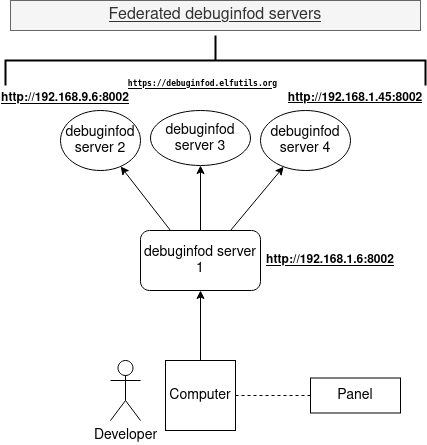
\includegraphics[scale=.375]{federeated_servers.png}
   %include image
   %include diagram
\end{frame}

\begin{frame}
   \frametitle{ Federeating debuginfod servers (cont.) }
   \begin{center}
   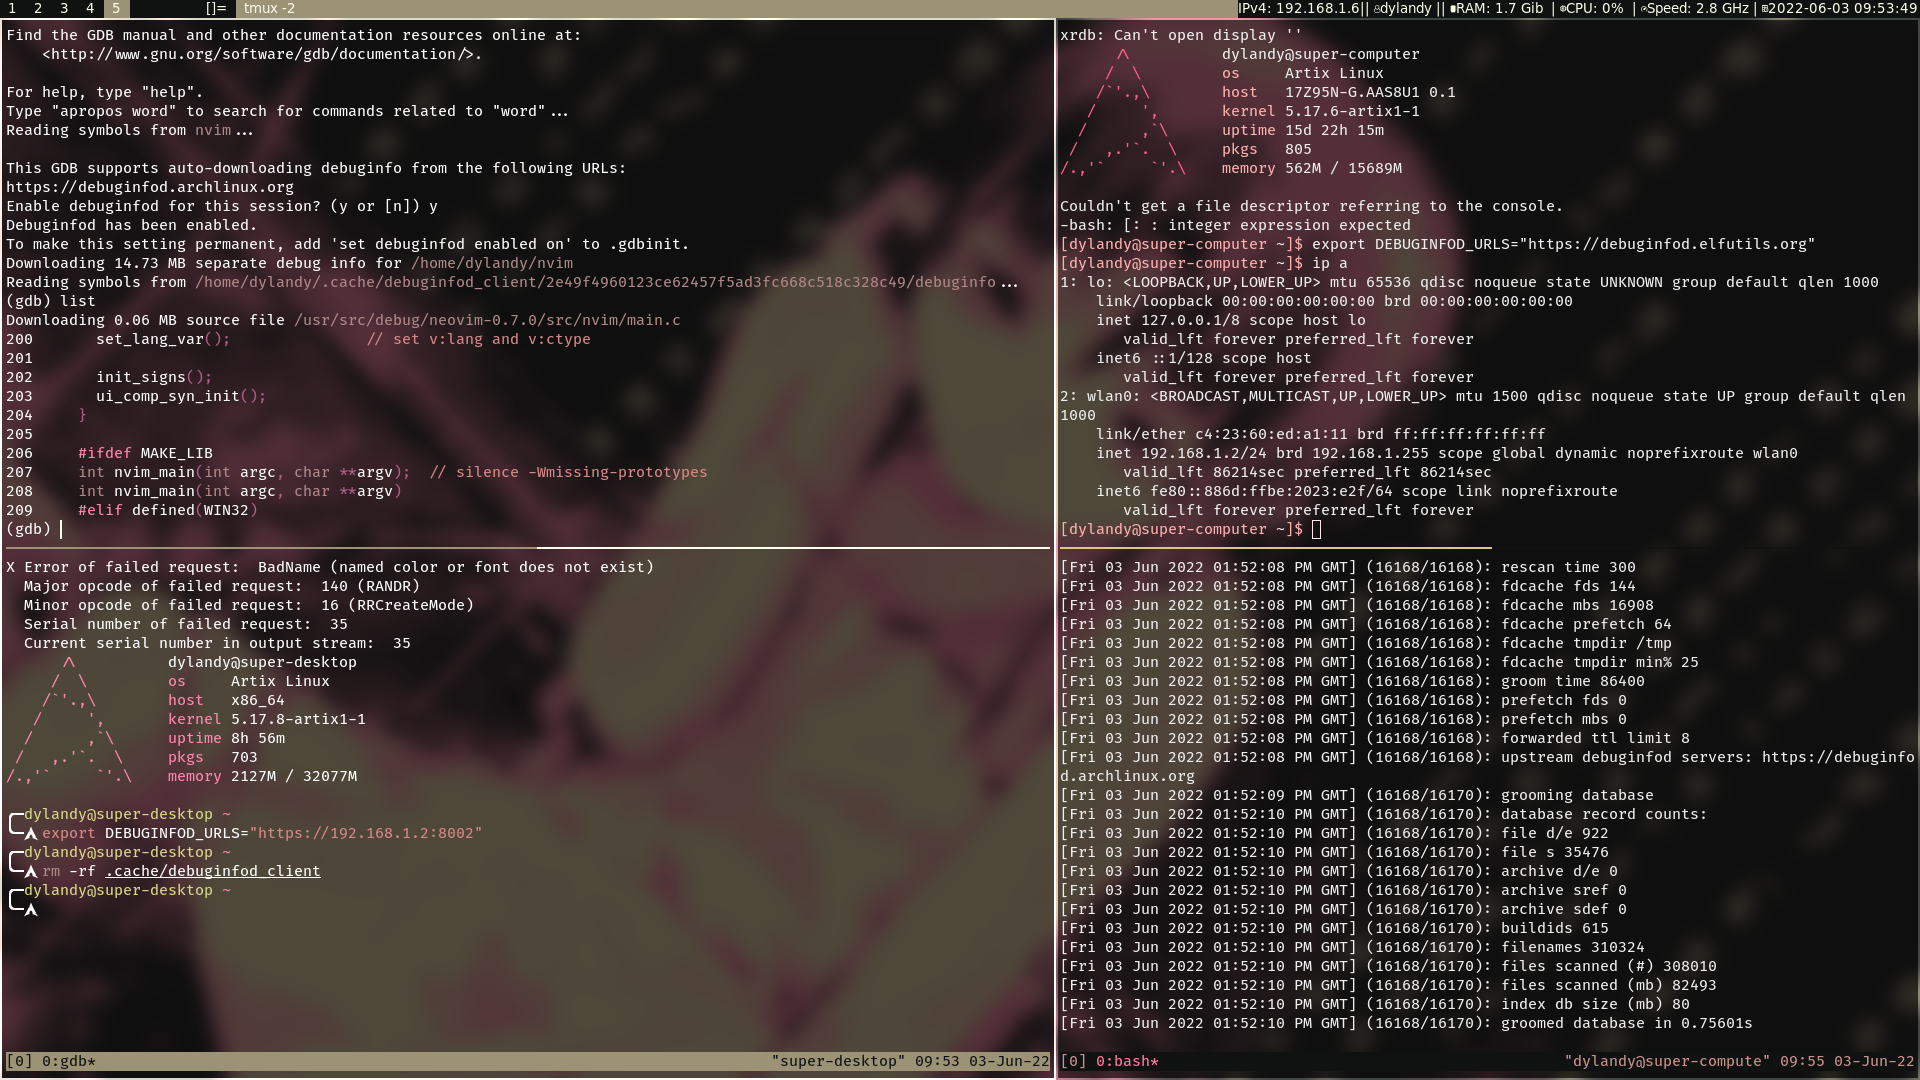
\includegraphics[scale=.175]{federated_ss.png}
   \end{center}
\end{frame}
\begin{frame}[fragile]
   \frametitle{ debuginfod-find}
   \begin{itemize}
      \item The \color{gray}\verb|debuginfod-find| \color{black}command allows the retrieval of debug artifacts, binary 
   executables, or sources without the use of gdb. The command simply calls for the type of file to 
   query and retrieve and the path to the binary or Build-ID. Additionally if a source is requested
   the path to the source also must be provided.
   \end{itemize}
   \fontsize{7pt}{10pt}\selectfont
   \color{gray}
   \begin{verbatim}
   debuginfod-find [debuginfo/executable/source] [path/to/file or Build-ID] [path/to/source]
   \end{verbatim}
   \fontsize{10pt}{10pt}\selectfont
   \begin{itemize}
      \item The requested file will be stored in the same directory as a normal successful 
         debuginfod query.
      \item Source files will be named by their path, with "\#\#" in place of "\//".
   \end{itemize}
   \color{gray}
   \begin{verbatim}
   ~/.cache/debuginfod_client/[Build-ID]/path##to##source.c
   \end{verbatim}

\end{frame}

\begin{frame}[fragile]
   \frametitle{ debuginfod with the Yocto Project}
   For versions after 3.4(honister) only 2 changes are needed for debuginfod
   to work on a build. Append the following the \verb|local.conf|:
   \begin{small}
   \begin{enumerate}
      \item \verb|PACKAGE_CONFIG_pn-elfutils-native="debuginfod libdebuginfod"|
      \item \verb|DISTROFEATURES += "debuginfod"|
   \end{enumerate}
   \end{small}
   Yocto Project has built in script for debuginfod to eliminate compatability issues. 
\end{frame}




\begin{frame}
   \frametitle{ Demo}
\end{frame}

\begin{frame}
   \frametitle{ Demo}
\end{frame}


\end{document}
